\clearpage \section{组合博弈论}
\subsection{P/N 分析}
\begin{itemize}
  \item P-Position: 必败态,指上一步 (Previous) 行动玩家必胜.
  \item N-Position: 必胜态,指下一步 (Next) 行动玩家必胜.
\end{itemize}

通过 P/N 分析可以从直接后继局面的 P/N 情况得出当前状态的 P/N 情况, 对于决策集合为空算败的游戏:

\begin{itemize}
  \item 无后继状态均为 P-Position.
  \item 如果所有后继均为 N-Position, 则当前状态为 P-Position.
  \item 若后继中存在 P-Position, 则当前状态为 N-Position.
\end{itemize}

P/N 状态可以指导游戏的进行, 一个处于 N-Position 的玩家应当向 P-Position 转移, 以将必败态留给对手.

P/N 分析只适用于单个游戏, 多个游戏的情况下 P/N 的结果无法直接相加, 此时需要用到其它数学工具.

\subsection{无偏博弈}
无偏博弈是一类双人游戏, 它满足以下条件:

\begin{itemize}
  \item 完全信息, 所有游戏者都能看到整个局势. 这排除了类似桥牌一类的游戏.
  \item 无随机行动. 所有行动都确定性地将目前局势转变到下一个局势.
  \item 在有限步行动之后按照规则游戏必将终止, 此时有唯一的一方成为赢家.
\end{itemize}

任何无偏博弈均可被抽象为一张有向无环图, 状态视为节点, 转移视为边. 所有的状态均可通过分析确认落在该状态的玩家是必胜或必败, 游戏只有胜败两种结局, 没有和.

\subsubsection{Sprague–Grundy 函数}
Sprague–Grundy 函数是一个将无偏博弈的局面映射为自然数的函数, 通过 SG 函数可以计算出某个无偏博弈是 P-Position 还是 N-Position.

定义 $\operatorname{mex}$ 函数为将自然数集合子集映射到单个自然数的函数, 其含义为第一个未在集合中出现的自然数: $\operatorname{mex}\mathbb S=\min\mathbb N\setminus\mathbb S$

\begin{itemize}
  \item 无后继的状态 SG 值均为 0.
  \item 有后继的状态 SG 值为所有后继状态 SG 值组成的集合的 $\operatorname{mex}$
\end{itemize}

SG 函数和 P/N 关系的映射为: SG 值为 0 的状态均为 P-Position, SG 值非 0 的状态均为 N-Position.

若一个游戏的某个局面可以被划分为多个互不干扰的子局面, 则其 SG 值为所有子局面 SG 值的异或和.

\subsubsection{Bash 游戏}
一堆 $n$ 枚石子, 两个玩家轮流操作, 每轮只能取 $1,\dots,k$ 枚, 无子可取败.

局面的 SG 值为 $n\bmod (k+1)$.

\subsubsection{Wythoff 游戏}
两堆 $n,m$ 枚石子, 两个玩家轮流操作, 每轮要不从两堆种取走相同个数的石子, 要不从其中一堆取走任意非零个数石子, 无子可取败.

SG 函数没有规律, 只能现场打表. 但是可以确认必败态的位置为 $\left\{\left(\lfloor k\phi\rfloor,\lfloor k\phi^2\rfloor\right):k\in\mathbb N\right\}$.

\subsubsection{Nim 游戏}
$n$ 堆石子, 两人轮流操作, 每轮只能选择其中一堆取走任意非零数量的石子, 无子可取败.

可以将每一堆视作两两之间互不干扰的子游戏. 则石子数为 $n$ 的子游戏的 SG 值为 $n$, 和游戏的 SG 值为所有石子堆石子个数的异或和.

\subsubsection{Staircase Nim 游戏}
阶梯游戏, 两人轮流操作, 每轮从一级阶梯选择非零数量的石子放到下一级, 无子可动败.

设最底下为第 0 阶, 则阶梯博弈等价于所有奇数编号堆石子组成的 Nim 游戏. 由于偶数阶移出的石子可以被直接移回下一个偶数阶, 所以不会产生影响.

\subsubsection{Lasker's Nim 游戏}
$n$ 堆石子, 两人轮流操作, 每轮选中一堆, 要不从中取走非零块, 要不将其分为非空的两堆.

可以将每一堆视作两两之间互不干扰的子游戏. 则 SG 函数值为 $\operatorname{SG}(0)=0$, 其它情况下 $\operatorname{SG}(4k)=4k-1$, $\operatorname{SG}(4k+1)=4k+1$, $\operatorname{SG}(4k+2)=4k+2$, $\operatorname{SG}(4k+3)=4k+4$, 其中 $k\in\mathbb N$.

\subsubsection{Moore's Nim-\(k\) 游戏}
$n$ 堆石子, 两人轮流操作, 每轮选中至少 1 堆至多 $k$ 堆, 从每堆中任意取非 0 石子, 无子可取败.

无 SG 函数准确表达, 但是可以确认必败态. 对于每个二进制位, 将每一堆石子的该位在模 $k+1$ 意义下相加, 若每一位得到的数均为 0, 则为必败态, 反之必胜态.

\subsubsection{Every-SG 游戏}
人为将多个游戏组合成一个游戏, 对于每一个存在后继的子游戏, 两个玩家均需要进行移动, 最终所有游戏均无子可动败.

显然必胜局面的子游戏需要尽量后延, 必败的子游戏要尽早结束. 那么考虑单个游戏的步数, 若到终态步数最长的游戏为奇数则当前状态为必胜态, 反之必败态.

\subsubsection{Take and Break 游戏}
1 堆石子, 两人轮流操作, 每轮移走一整堆, 添加两堆 (可空) 的石子堆, 无子可取败.

$\operatorname{SG}(n)$ 为第 $n$ 个 Odious 数. Odious 数是二进制位中 1 的个数为奇数的数, 如 1, 2, 4, 7, 8.

\subsubsection{最小元唯一的偏序集上的游戏}
不知名, 刘汝佳《训练指南》上给出.

给出一个只有唯一一个最小元的偏序集 (如正整数和整除关系, 矩形和完全包含关系), 两个玩家轮流删去元素, 若删去某元素, 则需要将所有比它小的元素一并删去.

只有空集必败, 其它情况均必胜. 考虑无最小元的情况, 若当前局面为必胜态, 则有无最小元无影响, 若当前局面为必败态, 则有最小元的相同局面可以先手除去最小元反转胜负.

\subsubsection{每轮最多移走一半石子}
不知名, 做题的时候碰到.

1 堆石子, 两人轮流操作, 每轮只能取走至少 1 枚至多一半的石子, 无子可取败.

显然 0 枚和 1 枚为必败态. 直接给出求 SG 函数代码.

\begin{lstlisting}
long sg(long a) {
  while (a & 1) a >>= 1;
  return a >> 1;
}
\end{lstlisting}

\subsection{Mis\`ere 游戏}
上文中所有的游戏均假定为无子可动者败, 也就是说无后继的状态败. 若规则改为无后继的状态胜利, 则无法直接使用 SG 函数是否为 0 判断 P/N-Position.

考虑原本意义的 SG 函数, Mis\`ere 游戏胜利条件为 (所有子游戏 SG 异或和为 0) \textbf{xor} (存在一个子游戏 SG 值大于 1).

\subsubsection{Mis\`ere Nim 游戏}
$n$ 堆石子, 两人轮流操作, 每轮只能选择其中一堆取走任意非零数量的石子, 无子可取胜.

胜利条件为 (所有石堆数目异或和为 0) \textbf{xor} (存在一堆石子数大于 1).

\subsubsection{Mis\`ere Moore's Nim-\(k\) 游戏}
$n$ 堆石子, 两人轮流操作, 每轮选中至少 1 堆至多 $k$ 堆, 从每堆中任意取非 0 石子, 无子可取胜.

胜利条件为 (所有二进制位 1 的数量 $\bmod (m+1)$ 为 0) \textbf{xor} (存在一堆石子数大于 1).

\clearpage
\subsection{翻硬币游戏}
带约束的翻硬币问题: 有 $n$ 枚硬币按行排列, 或正或反面朝上. 两个玩家轮流操作, 每轮翻转的硬币序列中最右侧那一枚必须为从正面翻转为反面.

可以认为每一枚初始朝上的硬币是一个单独的游戏.

\subsubsection{每轮只能翻一枚硬币}
显然和正面朝上的硬币数奇偶性有关.

\subsubsection{每轮只能翻转一枚或两枚硬币}
等价于 Nim 游戏, 左至右从 1 开始编号, 第 $n$ 枚正面朝上等价于一堆中有 $n$ 枚石子.

\subsubsection{每轮至多翻转三枚硬币}
左至右从 0 开始编号, 第 $n$ 枚正面向上的硬币等价于一个 $\operatorname{SG}(n)=2n+\operatorname{parity}(n)$ 的游戏.

其中 parity 是奇校验位函数, $\operatorname{parity}(n)$ 在 $n$ 的二进制表示中 1 的个数为偶数时候返回 1, 奇数返回 0 (即 \lstinline{!__builtin_parity(n)}).

\subsubsection{每轮翻转两枚距离 \(\le k\) 中的硬币}
左至右从 0 开始编号, 第 $n$ 枚正面向上的硬币等价于一个 $n$ 枚石子每轮最多取 $k$ 枚的 Bash 游戏. 翻转相邻的第 $k$ 个等价于取走 $k$ 枚石子.

\subsubsection{每轮翻转连续的 \(k\) 枚硬币}
左至右从 1 开始编号, 第 $n$ 枚正面向上的硬币等价于一个 $\operatorname{SG}(n)=[k\mid n]$ 的游戏.

\subsubsection{每轮翻转任意长度的连续一段硬币}
左至右从 1 开始编号, 第 $n$ 枚正面向上的硬币等价于一个 $\operatorname{SG}(n)=\lfloor\log_2n\rfloor+1$ 的游戏.

\clearpage
\subsection{Hackenbush 游戏}
所谓的有根链/树/图上删边问题. 给定一个有根链/树/图, 两人轮流删边, 每轮选择一条边删去, 然后将所有不与根连通的节点和边一并删去, 无边可删败.

\subsubsection{链上删边游戏}
一条长为 $n$ 的链等价于一堆石子数为 $n$ 的 Nim 博弈.

\subsubsection{树上删边游戏}
每个节点均有对应的 SG 值, 其中叶子节点的 SG 值为 0, 非叶子节点的 SG 值为其所有直接孩子节点 SG 值加一的异或和. 整棵树的 P/N 状态由根节点的 SG 值确定.

\subsubsection{图上删边游戏}
将环内有奇数条边的环缩成单点和一条挂出来的边, 偶数条的缩成单点, 化为树上删边.

\lstinputlisting{CGT/hackenbush.cc}

\subsection{\(k\) 倍动态减法}
一堆 $n$ 枚石子, 两人轮流操作. 首先确定一个游戏中不改变的数字 $k$, 然后开始游戏. 先手选择一个数字 $0<s_0<n$, 从石堆中取走这么多的石子. 之后双方轮流取走 $s_i$ 个石子, 满足 $0<s_i<ks_{i-1}$, 无子可取败.

当 $k=1$ 时, 必败态为 $n$ 等于 2 的幂次的局面. 当 $k=2$ 时, 必败态为 $n$ 等于 Fibonacci 数的局面. 对于更一般的 $k$, 可以使用以下代码 \lstinline{dynSubPPos} 计算出所有 P-Position.

生成的 P-Position 数据可以作为进制基底 ($k=0$ 二进制, $k=1$ Fibonacci 编码, 依此类推). 则必胜方的策略为每次取走当前 $k$ 对应的数列作为进制基底的编码下, 最低的 1 位对应的数字.

\lstinputlisting{CGT/dynamic-sub.hh}

\subsection{Nimber}
Nimber 是由非负整数 $\mathbb N$, 异或 $\oplus$ 和 Nim 积 $\otimes$ 组成的域. 另一个类似定义: 当数集范围为 $\{k\in\mathbb N:k<2^{2^n}\}$ 时, 该域即为 Galois 域 $\mathrm{GF}(2^{2^n})$. 该域可用于计算高维 Nim 游戏 SG 函数值.

\subsubsection{移棋子游戏 \uppercase\expandafter{\romannumeral1}}
一张棋盘上有数枚棋子, 二人轮流操作, 每轮选择一枚位于 $(n,m)$ 的棋子, 选择减少行或减少列, 将棋子移动到 $(n',m)$ 或 $(n,m')$, 其中 $0\le n'<n,0\le m'<m$. 棋子之间互不影响, 无子可动败.

容易证明, 每一枚位于 $(n,m)$ 的棋子相当于两堆石子数分别为 $n$ 和 $m$ 的 Nim 游戏, 所以每一枚棋子对应的 SG 值为 $n\oplus m$.

\subsubsection{移棋子游戏 \uppercase\expandafter{\romannumeral2}}
一张棋盘上有数枚棋子, 二人轮流操作, 每轮选择一枚位于 $(n,m)$ 的棋子, 选择一对整数 $(n',m')$ 满足 $(0\le n'<n)\land(0\le m'<m)$, 将位于 $(n,m)$ 的棋子移除, 并在棋盘 $(n',m)$, $(n,m')$ 和 $(n',m')$ 位置加入三枚棋子. 棋子之间互不影响, 无子可动败.

每一枚位于 $(n,m)$ 的棋子相当于一个子游戏, 其 SG 函数值为 $n\otimes m$. 根据 SG 函数的定义, $n\otimes m=\operatorname{mex}\{n'\otimes m'\oplus n'\otimes m\oplus n\otimes m':0\le n'<n,0\le m'<m\}$, 且 $\forall n,m:n\otimes0=0\otimes m=0$. 利用 $\otimes$ 的一些性质可以降低计算复杂度到 $O(\log^2\min\{n,m\})$, 见代码.

该式可以拓展到更高维, 若一张三维棋盘有棋子位于 $(n,m,k)$, 每次操作选择一个三元组 $(n',m',k')$ 满足 $(0\le n'<n)\land(0\le m'<m)\land(0\le k'<k)$, 将原棋子移除, 和二维棋盘类似地新增 7 枚由 $(n,m,k)$ 和 $(n',m',k')$ 确定的长方体 8 个角落上的 7 枚棋子. 则一枚位于 $(n,m,k)$ 的棋子的 SG 值为 $n\otimes m\otimes k$.

\lstinputlisting{CGT/nimber.hh}

\subsection{不平等博弈}

不平等博弈不属于无偏博弈, 和无偏博弈相比差别在于两个玩家在同一个局面的决策集可能不同, 因此不能使用 SG 函数解决. 但是仍有数学分析工具, 如 P/N 分析和超现实数.

\subsubsection{超现实数}

超现实数由递归定义, 一个超现实数由两个超现实数集合有序对构成, 记为 $\{\mathcal L|\mathcal R\}$, 要求 $\mathcal L$ 中的每个元素均小于 $\mathcal R$ 中的每个元素. 所有的实数均可映射入超现实数, 同一个超现实数会存在多种不同的表达.

定义 $0=\{|\}$, 正数 $1=\{0|\},2=\{1|\},\dots,n+1=\{n|\}$ 和负数 $-1=\{|0\},-2=\{|-1\},\dots,-n-1=\{|-n\}$, 于是将所有整数映射入超现实数.

定义 $\displaystyle\frac12=\{0|1\},\frac14=\left\{0\middle|\frac12\right\},\frac34=\left\{\frac12\middle|1\right\},\dots,\frac k{2^n}=\left\{\frac{k-1}{2^n}\middle|\frac{k+1}{2^n}\right\}$.

\begin{center}
  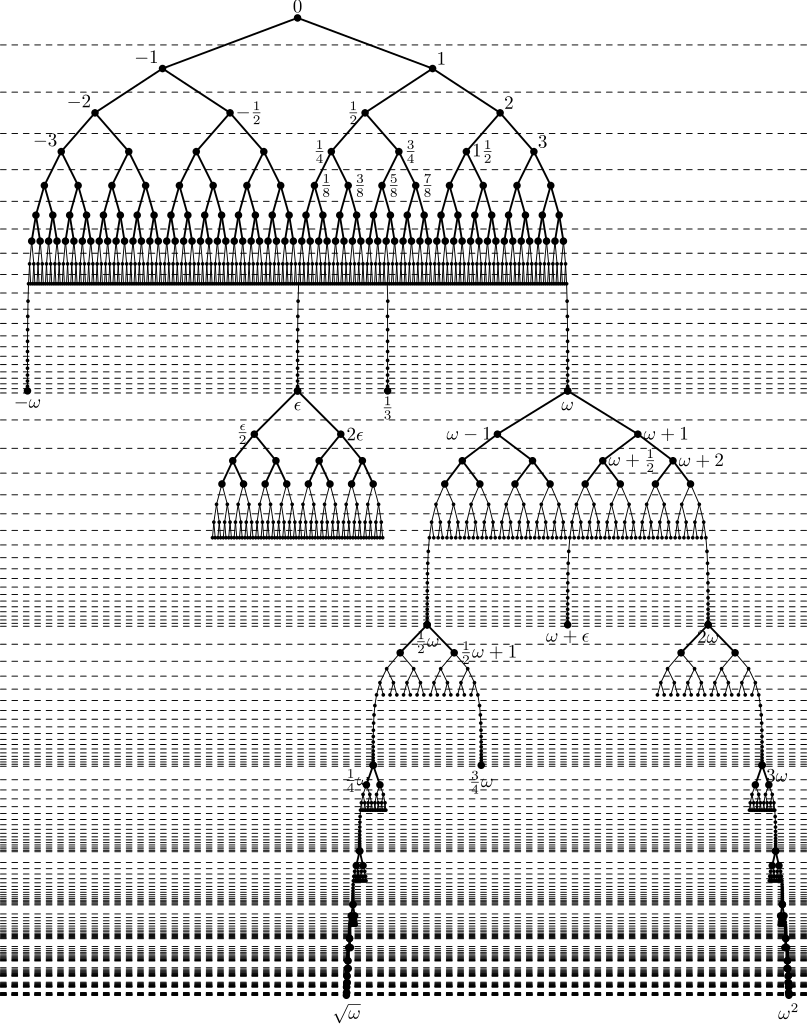
\includegraphics[scale=0.375,natwidth=811,natheight=1024]{CGT/811px-Surreal_number_tree.svg.png}
\end{center}

如上图建立超现实数树. 则有对于所有超现实数 $S=\{\mathcal L|\mathcal R\}$, 满足 $S=\{\max\mathcal L|\min\mathcal R\}$ $\max\mathcal L<S<\min\mathcal R$ 内, 且在上图中为最靠近根的那个节点对应的数.

迄今定义的超现实数已经可以用于解决不平等博弈问题, 其余定义均略去. 对于一个游戏, 可以将每个局面映射到一个扩展超现实数上, 所谓扩展, 是没有要求 $\mathcal L$ 中的所有元素均小于 $\mathcal R$ 中元素, 则可能会产生这种元素 $\{0|0\}$, 该元素不等于 0, 但是几乎等价于 0, 记作 $0\parallel\{0|0\}$.

称两个玩家分别为 L 和 R, 以如下方式递归地将所有局面映射为超现实数: 设 $\mathcal L$ 为玩家 L 可以一步达到的局面对应的超现实数集合, $\mathcal R$ 为玩家 R 可以一步到达的局面对应的超现实数集合, 则当前局面对应的超现实数为 $\{\mathcal L|\mathcal R\}$.

多个子局面对应的超现实数可以直接相加. 设某个局面为 $G$, 则胜败条件为:

\begin{itemize}
  \item $G>0$ 则 L 必胜.
  \item $G<0$ 则 R 必胜.
  \item $G\parallel0$ 则先手必胜.
  \item $G=0$ 则后手必胜.
\end{itemize}

\subsubsection{Blue-Red Hackenbush 游戏}
和 Hackenbush 游戏相比 Blue-Red Hackenbush 的不同点就是为每条边染上了红蓝两种颜色, 两个玩家分别只能删去属于自己的颜色的边. 通常来说由于树/图的状态难以保存转移, 因此只考虑链上的 Blue-Red Hackenbush.

下述代码中, 假设为 \lstinline{'L'} 的边为 L 玩家拥有的链边, 则返回值即为该链对应的超现实数.

\lstinputlisting{CGT/surreal.hh}

\subsubsection{Cutcake 游戏}
一块 $n\times m$ 的巧克力沿沟壑纵横切开, L 玩家只能横切, R 玩家只能纵切. 两人一刀会将一块巧克力切成两部分, 下一位切的只能从被切开的小块中选择进行横纵切. 不能切就算败.

本题状态对应的超现实数可以从 $n,m$ 简单求出, 直接给出求超现实数的代码.

\lstinputlisting{CGT/cutcake.hh}
